\section{Safety Critical Systems Development}
\label{sec:criticalSysDev}
As the capabilities of technology grows, so does the complexity and capabilities of mechanical and electrical systems. Many of these systems are safety critical; the loss of correct functioning leads to loss of life, substantial material or environmental damage, or large monetary losses. The development of such complex systems requires a process with clearly defined design and implementation phases which are subdivided into several sub-processes and phases. Certain sets of analyses are required for each of the phases and when the analyses provide satisfactory outcomes, the process transitions into the next phase. 

In general, each field relies on various interpretations of the development process. In the field of aerospace technologies, the Aerospace Recommended Practice (ARP) is what is commonly used. The Society of Automotive Engineers (SAE) is an association of engineers and professionals devoted to the standards that guide the development of transportation systems~\cite{SAE:ARP4761, SAE:ARP4754A}. 

\subsection{The V Model}
The development of safety critical systems is theoretically guided by the V model process as defined in ARP4754~\cite{SAE:ARP4754A}. The V model relates steps of the design phase with a post-implementation phase. It describes how the requirements are produced in the design phase and then how those requirements are verified against the implementation in the post-implementation phase. The left side of the V describes the requirements, architecture, and expected component behavior of the system (see Figure~\ref{fig:v1}). The right side of the V describes the evaluation of the system implementation in light of the requirements. 

\begin{figure}[!htb]
        \center{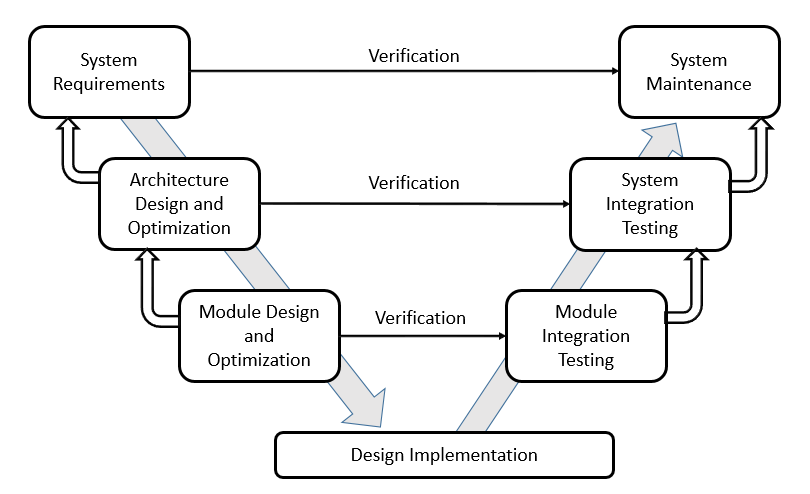
\includegraphics[width=0.85\textwidth] {images/v1.png}}
        \caption{\label{fig:v1} The V Model in System Development}
\end{figure}

\subsection{Model Based System Engineering and AADL}
Model-Based System Engineering (MBSE) designates engineering practices in which models of the system under development are central artifacts throughout the product's life cycle. These models help to define, design, analyze, and document the system under development~\cite{FeilerModelBasedEngineering2012}. 

Although models are not a perfect representation of the system, they provide knowledge and feedback in a faster and more cost-effective way than implementation alone; furthermore, they allow for simulation of complex interactions and serve as a guide for system implementation~\cite{INCOSE}. Depending on the modeling language, it is also possible to generate implementation code directly from the model itself, e.g.,~\cite{friedenthal2014practical,AADL_Standard,dabney2004mastering}. 

There are a number of modeling languages used in practice, for example SysML~\cite{friedenthal2014practical}, SCADE~\cite{abdulla2004designing}, Simulink~\cite{dabney2004mastering}, and AADL~\cite{FeilerModelBasedEngineering2012}. In this dissertation, we focus on one of these modeling languges: the Architecture Analysis and Design Language (AADL)~\cite{FeilerModelBasedEngineering2012}.

\subsubsection{Architecture Analysis and Design Language}
We are using the Architectural Analysis and Design Language (AADL) to construct system architecture models.  AADL is an SAE International standard language that provides a unifying framework for describing the system architecture for performance-critical, embedded, real-time systems~\cite{AADL_Standard,FeilerModelBasedEngineering2012}. From its conception, AADL has been designed for the design and construction of avionics systems.  Rather than being merely descriptive, AADL models can be made specific enough to support system-level code generation.  Thus, results from analyses conducted, including the new safety analysis proposed here, correspond to the system that will be built from the model.  
 
An AADL model describes a system in terms of a hierarchy of components and their interconnections, where each component can either represent a logical entity (e.g., application software functions, data) or a physical entity (e.g., buses, processors). An AADL model can be extended with language annexes to provide a richer set of modeling elements for various system design and analysis needs (e.g., performance-related characteristics, configuration settings, dynamic behaviors). The language definition is sufficiently rigorous to support formal analysis tools that allow for early phase error/fault detection.

For these reasons, we chose this modeling language as a foundational element of the model-based safety assessment research conducted for this dissertation.


\subsection{Traditional Safety Assessment Process}
ARP4754A, the Guidelines for Development of Civil Aircraft and Systems~\cite{SAE:ARP4754A}, provides guidance on applying development assurance at each hierarchical level throughout the development life cycle of highly-integrated/complex aircraft systems. It has been recognized by the Federal Aviation Administration (FAA) as an acceptable method to establish the assurance process. The safety assessment process is a starting point at each hierarchical level of the development life cycle and is tightly coupled with the system development and verification processes. It is used to show compliance with certification requirements and for meeting a company's internal safety standards. 

\begin{figure}[!htb]
        \center{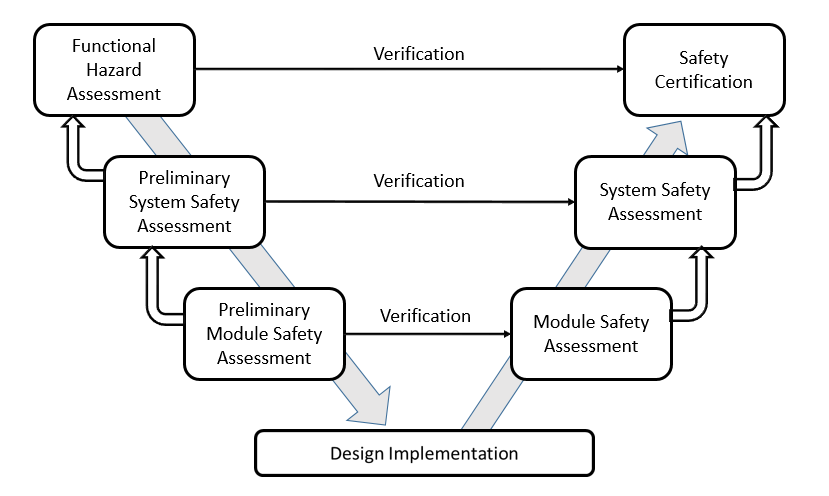
\includegraphics[width=0.85\textwidth] {images/v2.png}}
        \caption{\label{fig:v2} The V Model in Safety Assessment}
\end{figure}

The safety assessment shown in Figure~\ref{fig:v2} integrates each phase of the V model with analyses specific to system hazards and their severity. It also shows how these hazards should be addressed within the design phase. The safety assessment proess is defined in ARP4754A by the following phases:

\begin{description}
\item[Functional Hazard Assessment (FHA)] examines the functions of the system to identify potential functional failures and classifies the potential hazards associated with them. This includes identification of failure conditions, identifying the effects of those failures, classification of each failure condition, and assignment to safety objectives.

\item[Common Cause Analysis (CCA)] verifies and establishes physical and functional separation, isolation, and independence requirements between subsystems and verifies that these requirements have been met.

\item[Preliminary Aircraft Safety Assessment (PASA)] establishes aircraft safety requirements and provide a preliminary indication that the aircraft can meet those safety requirements.

\item[Preliminary System Safety Assessment (PSSA)] examines the proposed architecture(s) to determine how failures could cause the failure conditions determined by the FHA. The objective is to complete the safety requirements of an aircraft or system and show that the proposed system architecture satisfies the safety requirements. The PSSA is an iterative process that is performed at multiple stages of system development. 

\item[Fault Tree Analysis (FTA)] is performed to find combinations of faults that lead to the violation of a safety requirement. The fault tree itself shows the logical relation between the sets of faults and the violation of a safety requirement.

\item[Common Mode Analysis (CMA)] analyzes designs and implementations for elements that may defeat the redundancy
or independence of functions within the design, i.e. if elements are shown as independent in FTA, make sure they are truly independent in the system under consideration.

\item[Failure Modes and Effect Analysis (FMEA)] aims at finding the causality relationship between sets of faults, intermediate events, and undesired states in the system. Usually this is represented in tabular form and called an \textit{FMEA table}.

\item[Aircraft Safety Assessment (ASA)/System Safety Assessment (SSA)] verifies that the system (or aircraft), as implemented, meets the safety requirements specified by the PSSA.

\end{description}

\subsection{Model Based Safety Assessment}
\label{subsec:mbsa}

The lack of precise models of the system architecture and its failure modes often forces safety analysts to devote significant effort to gathering architectural details about the system behavior from multiple sources. Furthermore, this investigation typically stops at system level, leaving software function details largely unexplored. Typically equipped with the domain knowledge about the system, but not detailed knowledge of how the software applications are designed, practicing safety engineers find it a time consuming and involved process to acquire the knowledge about the behavior of the software applications hosted in a system and its impact on the overall system behavior. A diagram of this process is shown in Figure~\ref{fig:proposed_safety_process}.

\begin{figure}[h]
	\centering
	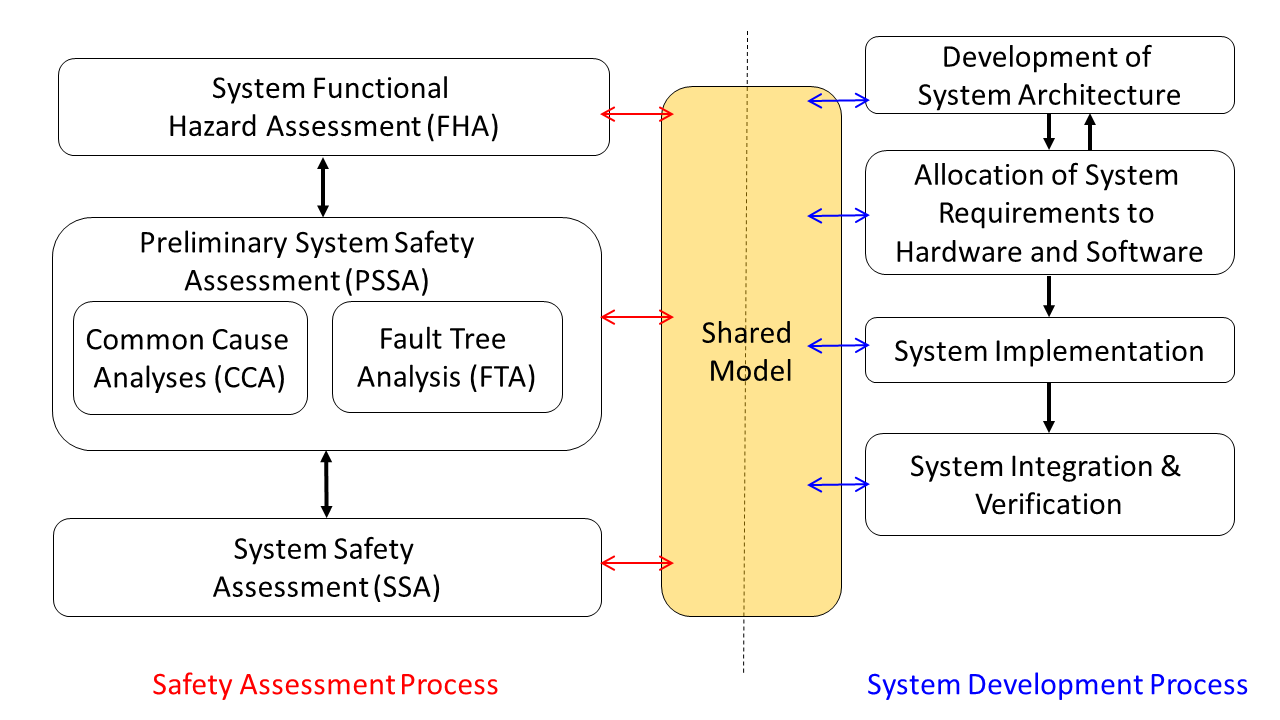
\includegraphics[trim=0 5 0 5,clip,width=0.85\textwidth]{images/process3.png}
	\caption{Use of the Shared System/Safety Model in the ARP4754A Safety Assessment Process}
	\label{fig:proposed_safety_process}
\end{figure}

Industry practitioners have come to realize the benefits of using models in the safety assessment process, and a revision of the ARP4761 to include Model Based Safety Analysis (MBSA) is under way. 

\subsection{Suggested Model Based Safety Assessment Process Supported by Formal Methods}
We propose a model-based safety assessment process backed by formal methods to help safety engineers with early detection of the design issues.  This process uses a single unified model to support both system design and safety analysis; this is shown in Figure~\ref{fig:SACycle1} and is based on the following steps:

\begin{enumerate}
	\item System engineers capture the critical information in a shared model:  high-level hardware and software architecture, nominal behavior at the component level, and safety requirements at the system level.
	\item System engineers use a model checker to check that the safety requirements are satisfied by the nominal design model. 
	\item Safety engineers augment the nominal model with the component failure modes. In addition, safety engineers specify the fault hypothesis for the analysis which corresponds to how many simultaneous faults the system must be able to tolerate.
	\item Safety engineers use a model checker to analyze if the safety requirements and fault tolerance objectives are satisfied by the design in the presence of faults. If the design does not tolerate the specified number of faults (or probability threshold of fault occurrence), then the tool produces counterexamples or minimal sets of fault combinations that can cause the safety requirement to be violated.
	\item The safety engineers examine the results to assess the validity of the fault combinations and the fault tolerance level of the system design. If a design change is warranted, the model will be updated with the latest design change and the above process is repeated.
\end{enumerate}

\begin{figure}[h]
	\begin{center}
		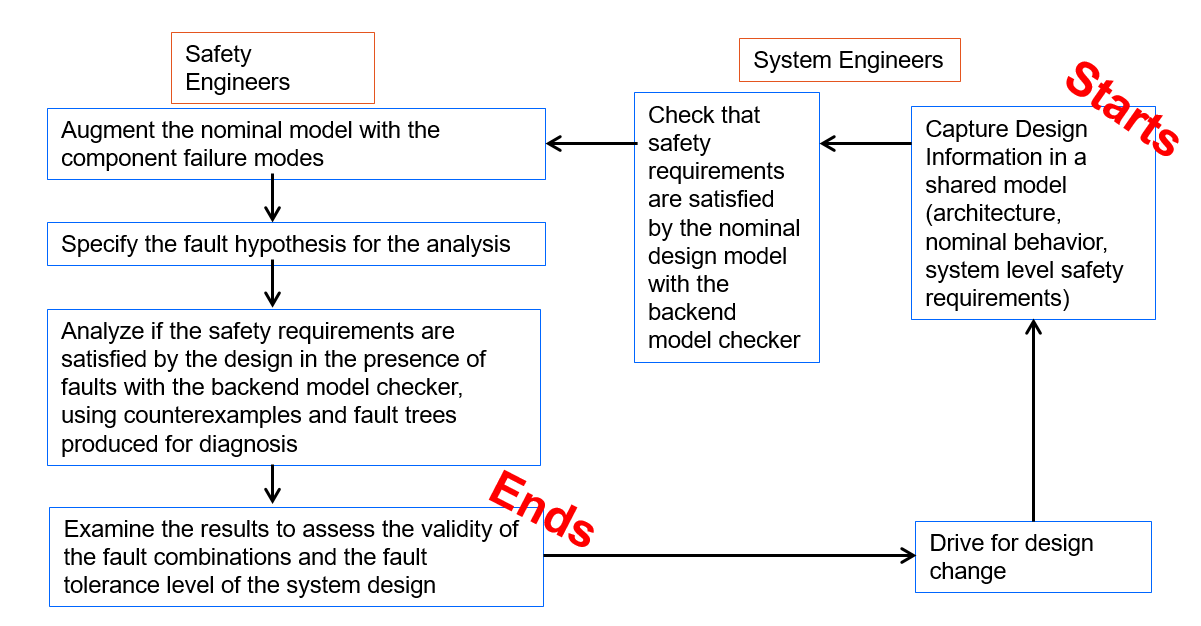
\includegraphics[width=\textwidth]{images/SACycle.PNG}
	\end{center}
	\caption{Proposed Steps of the Safety Assessment Process}
	\label{fig:SACycle1}
\end{figure}

These steps can be viewed as a cyclical process that involves both the system development engineers and the safety engineers of the system. Figure~\ref{fig:SACycle1} shows these steps within the context of the start and end of a project. 

\danielle{Add a bit more information here - pull from the MBSE project for IRAD. Include reasons why this approach is better, how it will help safety analysts, how it benefits the field as a whole. Then lead into the next sections with a statement about model checking, verification, etc.}
subsection{Critical System Development Artifacts}
\label{subsec:crisysArtifacts}












\begin{comment}
ARP4754A, the Guidelines for Development of Civil Aircraft and Systems~\cite{SAE:ARP4754A}, provides guidance on applying development assurance at each hierarchical level throughout the development life cycle of highly-integrated/complex aircraft systems. It has been recognized by the Federal Aviation Administration (FAA) as an acceptable method to establish the assurance process. The safety assessment process is a starting point at each hierarchical level of the development life cycle and is tightly coupled with the system development and verification processes. It is used to show compliance with certification requirements and for meeting a company's internal safety standards. 

ARP4761, the Guidelines and Methods for Conducting Safety Assessment Process on Civil Airborne Systems and Equipment~\cite{SAE:ARP4761},  identifies a systematic means to show compliance. Among the industry accepted safety assessment processes are Preliminary System Safety Assessment (PSSA) and System Safety Assessment (SSA). PSSA evaluates the system design and defines safety requirements. SSA evaluates the implemented system to show that safety requirements defined in the PSSA are in fact satisfied.

A prerequisite of performing the safety assessment is understanding how the system is intended to work, primarily focusing on the integrity of the outputs and the availability of the system. The safety engineers then use the acquired understanding to conduct safety analysis, construct safety analysis artifacts, and compare the results with established safety objectives and requirements.
Typically equipped with the domain knowledge about the system, but not detailed knowledge of how the software applications are designed, practicing safety engineers find it a time consuming and involved process to acquire the knowledge about the behavior of the software applications hosted in a system and its impact on the overall system behavior.
Industry practitioners have come to realize the benefits of using models in the safety assessment process, and a revision of the ARP4761 to include Model Based Safety Analysis (MBSA) is under way.
Figure~\ref{fig:proposed_safety_process} presents our proposed use of a single unified model to support both system design and safety analysis. It describes both system design and safety-relevant information 
that are kept distinguishable and yet are able to interact with each other. The shared model maintains a living model that captures the current state of the system design as it moves through the development lifecycle, allowing all participants of the ARP4754A process to be able to communicate and review the system design. Safety analysis artifacts can be generated directly from the model, 
providing
the capability to more accurately analyze complex systems.

\begin{figure}[t!]
	
	\centering
	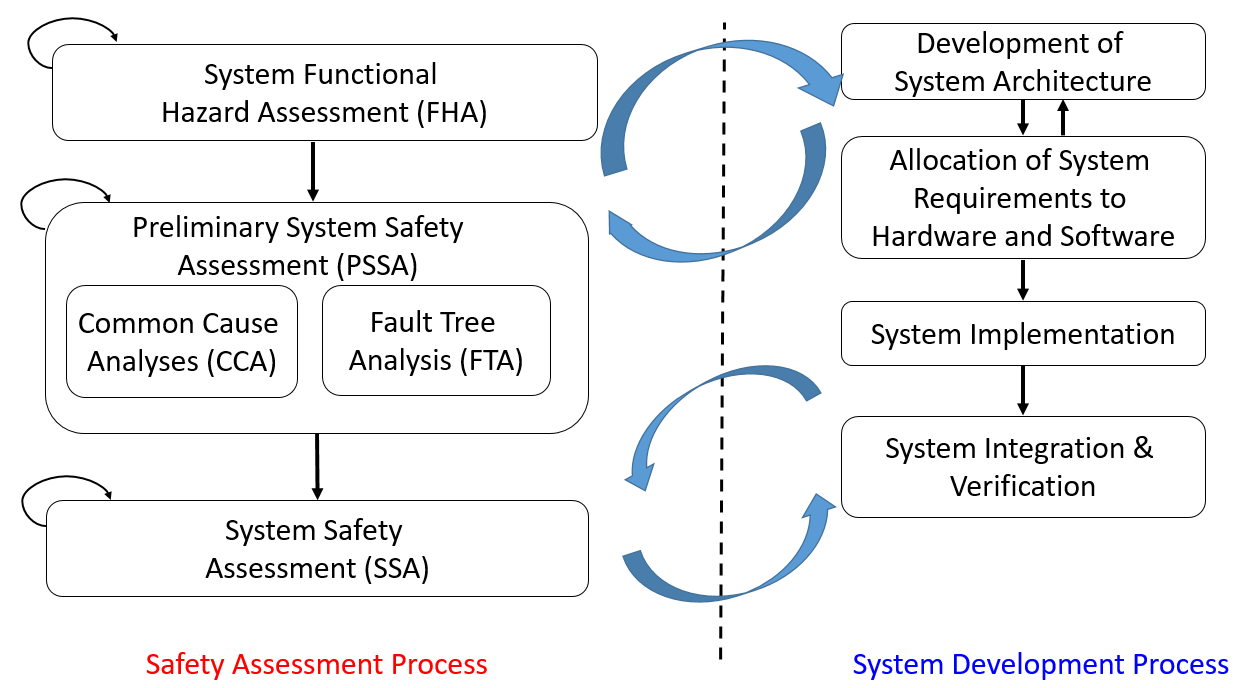
\includegraphics[trim=0 5 0 5,clip,width=0.85\textwidth]{images/process1.png}
	
	\caption{The ARP4754A Safety Assessment Process}
	\label{fig:safety_process}
\end{figure}

\begin{figure}[t!]
	
	\centering
	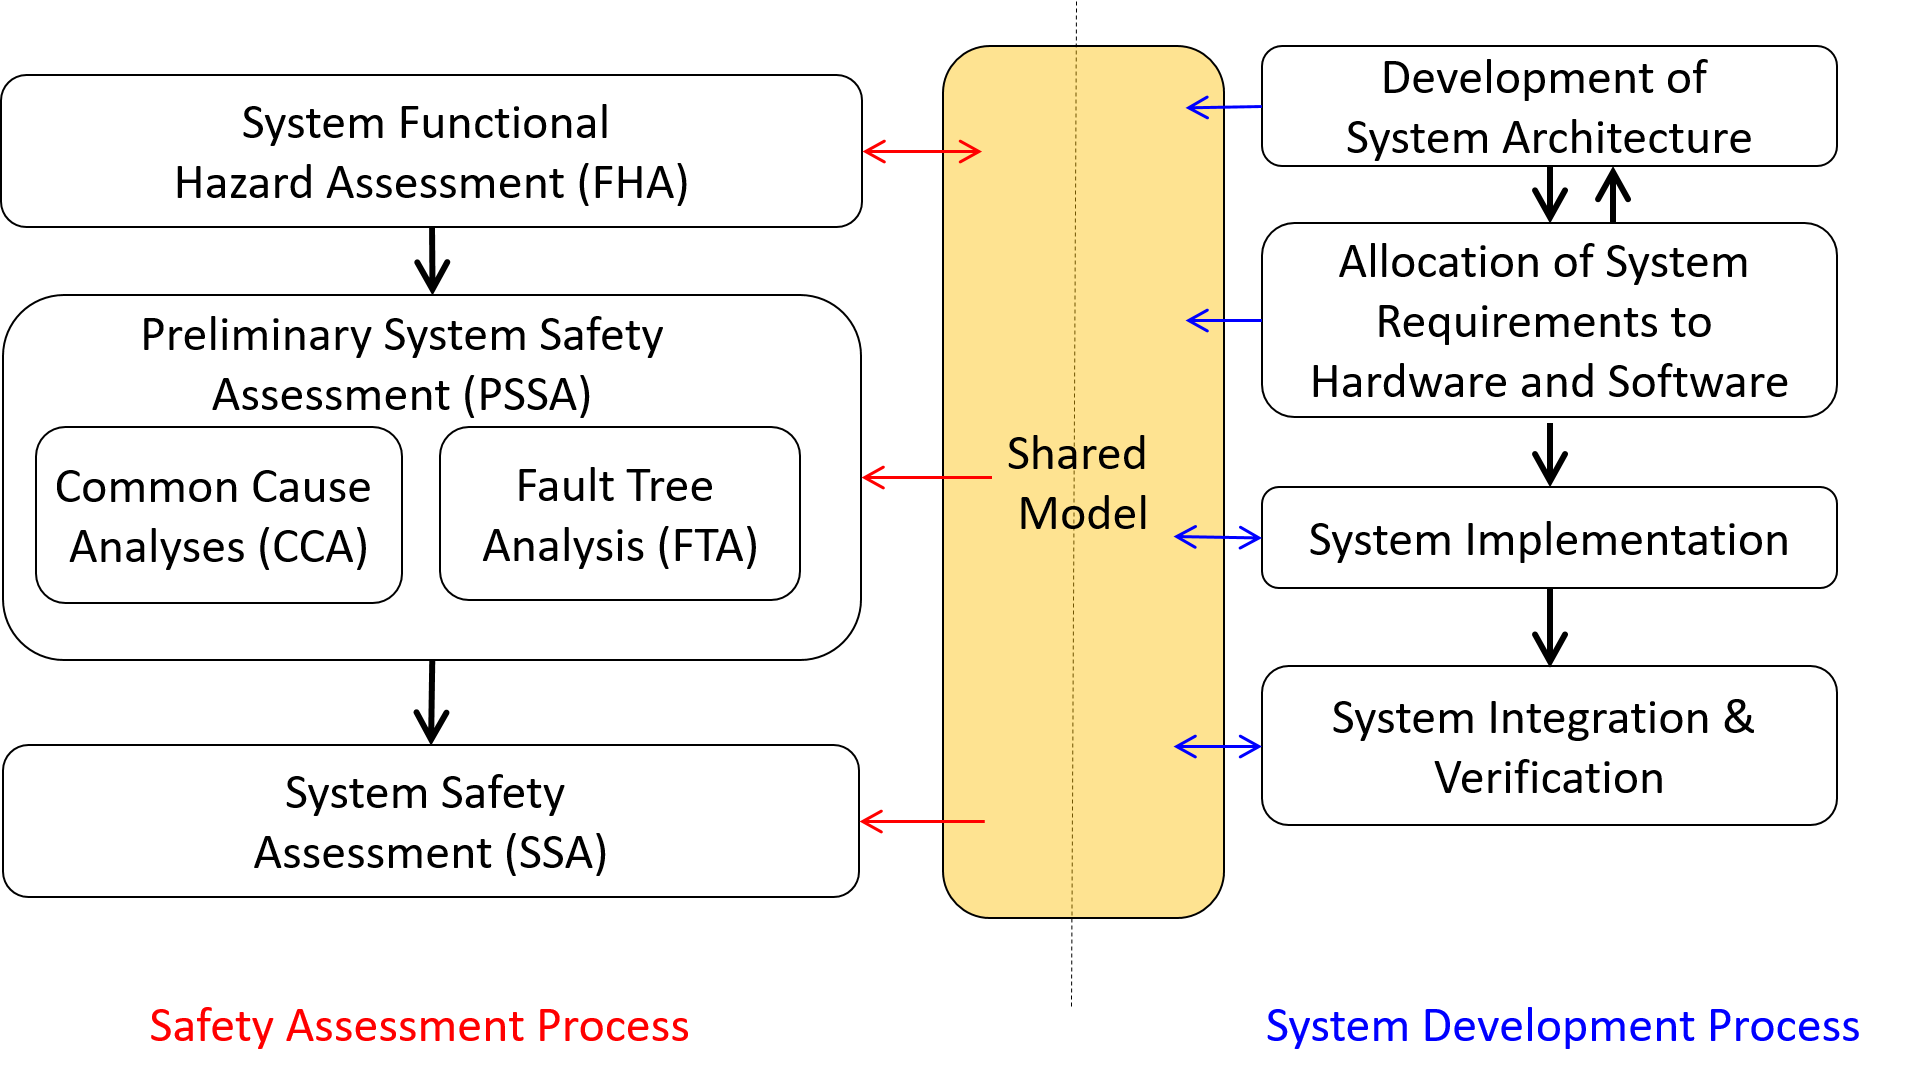
\includegraphics[trim=0 5 0 5,clip,width=0.85\textwidth]{images/process2.png}
	
	\caption{Use of the Shared System/Safety Model in the ARP4754A Safety Assessment Process}
	\label{fig:proposed_safety_process}
\end{figure}
\end{comment}